\subsection{Detection algorithm}
The purpose of the detection algorithm is to detect potentially too exposed devices. It analyzes the LoRa traffic, keeps track of all the detected DevAddress, and uses a pattern-matching strategy to verify if two collected DevAddress could be associated with the same ED.

\vspace{5mm}

In detail, the detection algorithm uses a vector \(\ C \) to store all the identified patterns. It contains a series of elements \(\ P_{a} \), where \(\ a \) is the current DevAddress associated to an ED, and \(\ P_{a} = \{ s_{1}, ..., s_{n} \} \) is the pattern the device follows. Since different patterns necessarily describe distinct EDs, in \(\ C \), there cannot be two tuples denoting the same device. In other words, let \(\ E \) be the set of all the ED that currently join the network, we have:
\[\ length(C) \subseteq length(E ) \]
The vector \(\ C \) allows checking if a given device, represented by its current DevAddres \(\ a \), already exchanged messages in the network. When the detection algorithm reads a new packet with DevAddress \(\ a \), it observe if the condition \(\ P_{a} \in C \) occurs. If \(\ P_{a} \notin C \) and this happens after the interception of a Join-request message, PIVOT  cannot establish \textit{a priori} the nature of the device associated to \(\ a \). It initiates a pattern-matching process to compute if \(\ a \) belongs to a new device or a re-joined one, trying to achieve this task in the shortest time possible. In this way, in the case of potential matching, the algorithm minimizes the delay in triggering the alert.

\vspace{5mm}

Intercepting a Join-request message is a crucial part of the detection process. It permits PIVOT to comprehend which addresses it needs to investigate and which patterns we should use for the matching procedure. The pattern \(\ P_{a} \notin C \), associated with an unknown address \(\ a \), should \textit{not} be compared with all the other patterns of \(\ C \). We must exclude from our analysis all that pattern related to these two classes of addresses:

\vspace{3mm}
\begin{itemize}
	\item All the addresses collected after the Join request, which have been noticed also before the Join-request. They are associated with devices that never disconnect from the network.
	\item All the other unknown addresses received after the Join-request, since a new device that joins the network has not more than one DevAddr.
\end{itemize}
\vspace{3mm}

The algorithm follows two sequential steps, called \textit{Pre-Join} procedure and \textit{Main} procedure. Figure \ref{fig:pre_main} illustrates the two procedures. Let \(\ t_{0} \) the timestamp of the first packet received by PIVOT after its activation and \(\ t_{f} \) the timestamp of the first Join-request packet. The Pre-Join procedure takes place in the time window \(\ t_{f} - t_{0} \) and the Main procedure starts after the reception of the first Join-Request message, at \(\ t_{f} \). In the next sections, we are going to examine these two steps in detail.

\begin{figure}[H]
    \centering
    \vspace{4mm}
    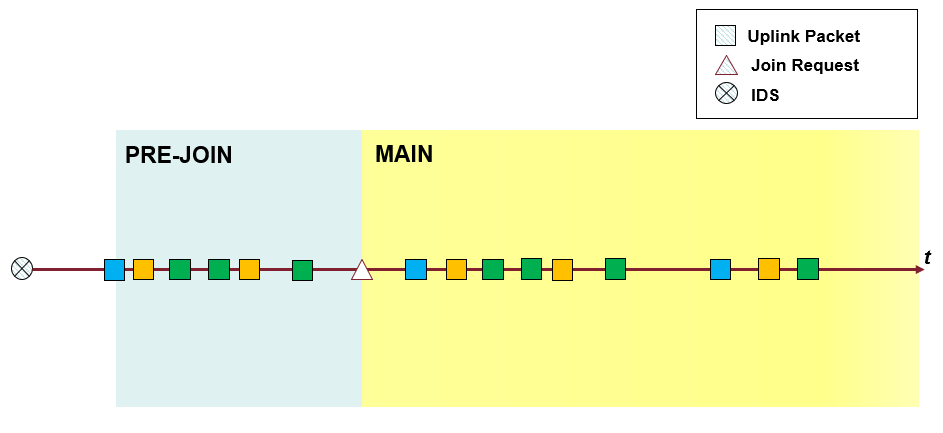
\includegraphics[width=0.7\linewidth]{images/pivot/pre-main.PNG}
    \caption{Representation of the time windows of the Pre-Join and Main procedures}
    \label{fig:pre_main}
\end{figure}
\vspace{5mm}

\begin{mintedbox}[samepage]{python}
def __pre_join(self, p):
    devaddr = p.dev_addr

    if devaddr in self.confirmed:
        self.confirmed[devaddr].update(p.t)
    else:
        self.confirmed[devaddr] = Pattern(p.t)
\end{mintedbox}
\subsubsection{Main procedure}
After the first Join-request message, the detection algorithm can no longer guarantee that a packet \(\ p \) with DevAddress \(\ a \) such that \(\ P_{a} \notin C \) necessarily belongs to a new, unregistered device. This time we have to consider also the hypothesis that the address \(\ a \) belongs to a  re-joined device. In detail, for each DevAddress \(\ a \), we have:

\vspace{3mm}
\begin{enumerate}
	\item \(\ P_{a} \in C \). \(\ a \) refers to a known ED, and it associated to a known pattern.
	\item \(\ P_{a} \notin C \). \(\ a \) refers to an unknown ED. The algorithm must recognize if it is belongs to a new device or an old one that re-joined the network.
\end{enumerate}
\vspace{3mm}

When the second scenario occurs, as in the Pre-Join procedure, a new pattern \(\ P_{a} \) is initialized. However, this time the pattern is not put in \(\ C \), but in a new vector, called \(\ U \), until the algorithm finds out if the address \(\ a \) represents a new device or not. Finally, the algorithm initialized the list \(\ TA_{a} \gets C \) of \textit{potential} patterns which could match with \(\ P_{a}\).

\vspace{5mm}

After the initialization of \(\ P_{a} \), each time the system receives as input a new packet \(\ p \) with the same address \(\ a \) and a new timestamp \(\ t \), the algorithm updates \(\ P_{a} \gets U \) and compares it with the patterns of \(\ TA_{a} \). Initially, the \(\ TA_{a} \gets verified(C) \) i.e. is it is composed of all the elements of C whose patterns is complete (then, with \textit{verified} flag set to \texttt{True}). After the updating of \(\ P_{a} \), three situations can occur:

\vspace{3mm}
\begin{enumerate}
	\item \(\ P_{a} \) doesn't match any element of \(\ TA_{a} \).
	\item The chain of \(\ P_{a} \) is a subset of one o more chains of the patterns of \(\ TA_{a} \).
	\item \(\ P_{a} \) matches \textit{exactly} with one o more elements of \(\ TA_{a} \).
\end{enumerate}
\vspace{3mm}

When the first scenario occurs, the DevAddress \(\ a \) necessarily represents a new ED. \(\ TA_{a} \) is erased from the storage and \(\ P_{a} \) is removed from \(\ U \) to be appended in \(\ C \). 

\vspace{5mm}

On the contrary, in the second case the chain of segments of \(\ P_{a} \) matches with the \textit{subchain} of one o more patterns of \(\ TA_{a} \). This implies that the chain of \(\ P_{a} \) may still be incomplete. Then the algorithm left \(\ P_{a} \) in the vector \(\ U \) and remove from \(\ TA_{a} \) all that pattern with which \(\ P_{a} \) don't match. 

\vspace{5mm}

In the last scenario, since there is a match between \(\ P_{a} \) and another pattern \(\ P_{b} \), most likely the associated addresses \(\ a \) and \(\ b \) belong to the same device. The algorithm inserts the \(\ P_{a} \) in a reservated vector, called \(\ Q \). When PIVOT will receive a new packet with DevAddress \(\ a \) such that \(\ P_{a} \in Q \), the algorithm starts the \textit{quarantine} subroutine, that will definitively confirm or reject the match between \(\ P_{a} \) and \(\ P_{b} \).

\vspace{3mm}
\begin{algorithm}
    \caption{Main procedure}
    \begin{algorithmic}[1]
        \If{$P_{a}$ n $C$}
            \State $P.update(t)$
        \Else
            \If{$P_{a}$ in $U$}
                \State $P.update(t)$
                \If{$P_{a}$ in $Q$}
                    \State quarantine procedure
                \EndIf
                \ForAll{$P_{ta}$ in $TA(a)$}
                    \If{$match(P_{a}, P_{ta})$}
                        \State $Q \gets P_{a}$
                    \Else
                        \State $TA(a).remove(P_{ta})$
                    \EndIf
                \EndFor
                \If{$TA(a)$ is empty}
                    \State new device
                    \State $C \gets P_{a}$
                \EndIf
            \Else
                \State $P \gets newPattern(a)$
                \State $U(a) \gets P$
                \State $TA(a) \gets verified(C)$
            \EndIf
        \EndIf
    \end{algorithmic}
\end{algorithm}

\newpage

\vspace{5mm}
\subsubsection{Quarantine}
\begin{figure}[t]
    \centering
    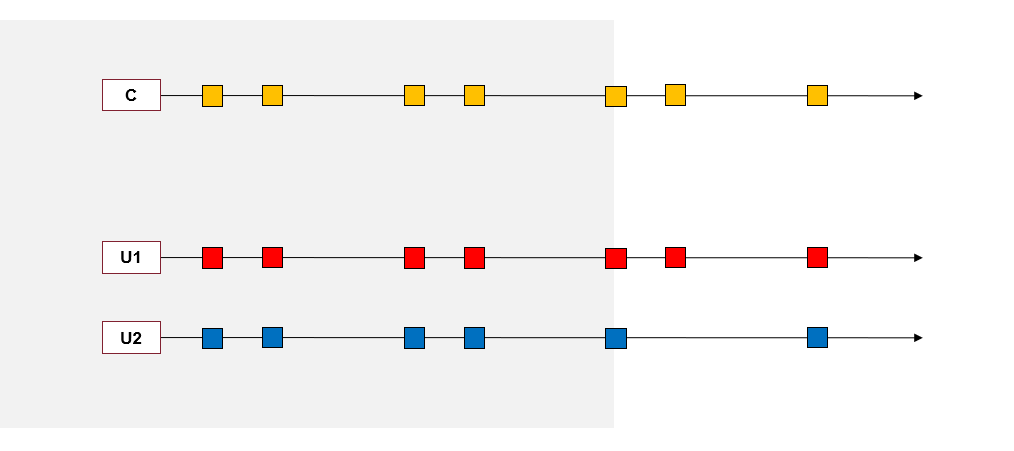
\includegraphics[width=0.7\linewidth]{images/pivot/quarantine.PNG}
    \caption{This example reports the two scenarios that can occur in the quarantine subroutine. In the first case, after updating the pattern \(\ U1 \), PIVOT confirms that \(\ U1 \) and \(\ C \) are linked to the same ED. In the second case, after updating the pattern \(\ U2 \), PIVOT confirms that \(\ U2 \) is associated to a new ED.}
    \label{fig:quarantine}
\end{figure}
When the incoming packet \(\ p \) has a DevAddress \(\ a \) such that \(\ P_{a} \in Q \), it means that \(\ P_{a} \) matches exactly with another pattern \(\ P_{b} \). The objective of the quarantine subroutine is to confirm this match or, on contrary, to demonstrate that \(\ P_{a} \) and \(\ P_{b} \) are linked to different EDs. Given the timestamp \(\ t \) of \(\ p \), the algorithm updates \(\ P_{a} \) and checks if \(\ P_{b} \) and \(\ P_{a} \) still match. If so, PIVOT triggers the \texttt{alert} the operator. If not, \(\ P_{a} \) belongs to a new device, then \(\ P_{a} \) moves from \(\ U \) to \(\ C \). The figure \ref{fig:quarantine} illustrates the two scenarios that can occur in the quarantine subroutine. Before of this step, the pattern \(\ C \) matches with both \(\ U1 \) and \(\ U2 \). In the first case, after updating \(\ U1 \) with the current timestamp \(\ t \), the algorithm confirms that \(\ U1 \) and \(\ C \) still matches. In the second case, after updating \(\ U2 \), the algorithm concluded that it represents the pattern of another device.

\vspace{3mm}
\begin{algorithm}[h!]
    \caption{Quarantine}
    \begin{algorithmic}[1]
        \State $P_{a} \gets U$
        \State $P_{b} \gets TA_{a}$
        \State $P_{a}.update(t)$
        \If{$match(P_{a}, P_{b})$}
            \State alert
        \Else
            \State new device
            \State $C \gets P_{a}$
        \EndIf
    \end{algorithmic}
\end{algorithm}
\vspace{5mm}

\newpage

\subsection{Metrics for operator}
PIVOT supports the network operator in its routine operations, providing a series of statistical metrics that illustrate the current state of the administered network.

\subsubsection{Number of Joins (NoJ)}
The Number of Joins (NoJ) represents the overall \textit{Join-request} messages intercepted and registered by PIVOT over the time. Generally, in LoRaWAN there is a \textit{peak} of Join-requests only in the starting phase when the operator registers and activates all the devices that will operate in the network. All Join-requests following this peak denote the insertion of new devices or the reconnection of old ones, two uncommon events. A too high value of NoJ might indicate the malfunction of one or more devices that are disconnecting and reconnecting continuously from the network. As demonstrated, sending a Join-request message could involve the expose the addresses of the device to unauthorized parties, then operator should avoid that the EDs send too many messages of this type.

\vspace{3mm}
\begin{figure}[H]
    \centering
    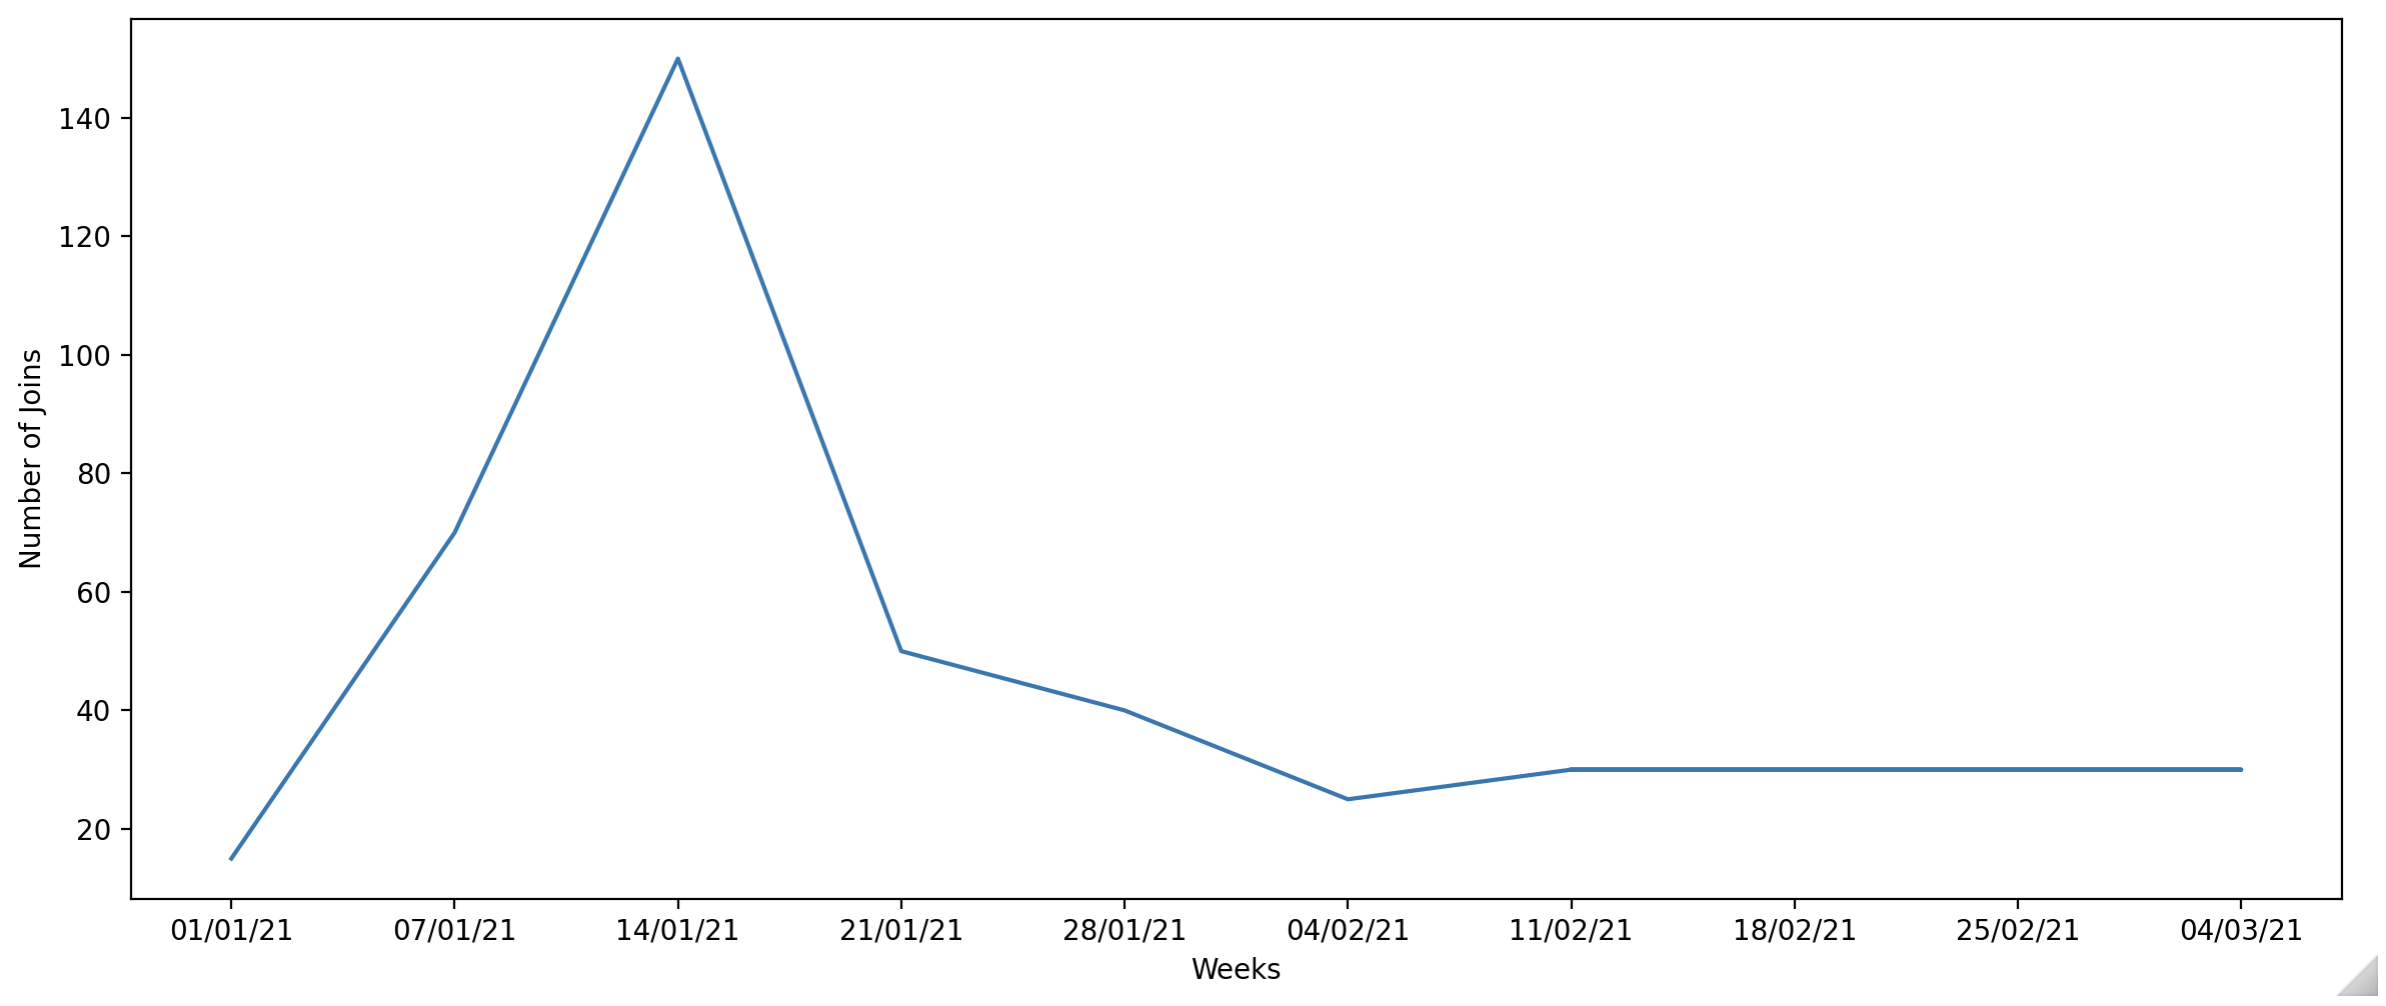
\includegraphics[width=0.7\linewidth]{images/pivot/NoJ.png}
    \caption{This plot reports an example of NoJ/weeks of a LoRaWAN network without anomaly devices. There is a peak only in the initial phase.}
    \label{fig:noj}
\end{figure}
\vspace{3mm}

\subsubsection{Number of Detected Devices (NoDD)}
The Number of Detected Devices (NoDD) describes the current amount of devices classified by PIVOT as vulnerable. These EDs, that re-joined the network at least once, have a too predictable pattern that could disclose their sensible characteristics, such as the identifiers, to external eavesdroppers. NoDD is updated each time PIVOT triggers the alert to the operator. This metric depends on the \textit{accuracy} of the detection algorithm of PIVOT, which may \textit{misclassify} some devices or miss capturing all vulnerable ones.

\subsubsection{Number of Unique Devices (NoUD)}
The Number of Unique Devices (NoUD) is the number of ED registered by PIVOT. These devices have sent at least one message to the server, exposing their DevAdress. NoUD does \textit{not} represent the total amount of devices of the network but only those that have transmitted packets since PIVOT was turned on. NoUD indicates the number of \textit{currently active} devices.

\subsubsection{Percentage of Detected Devices (PoDD)}
The Percentage of Detected Devices (PoDD) is a value in the range [0, 1] and represents the ratio between \textit{NoDD} and \textit{NoUD}. It provides a clear view of the network, showing exactly how many devices are vulnerable among all those present. Since it is not unusual for LoRa devices to generate periodic traffic, the PoDD value is generally always greater than zero. Using this metric, the operator can establish the \textit{maximum} permissible percentage of exposed devices, according to the dimension of the network. For example, in the case of environments made by a consistent number of devices, the management becomes more complex, and it is almost impossible to handle all the devices exposed. In this case, the goal could be to reduce the value of \textit{PoDD} whenever possible.